% =====================================================================
%  Introduction to Deep Learning — Class 28
%  Topic (course plan): Recurrent Neural Network
%  Subtopic (course plan): LSTM and Gated RNNs
%  Sources (course plan): Jurafsky & Martin Ch. 13 (Ch. 14 in the
%    August 2026 draft), Goodfellow Ch. 10
%
%  Class 27 treated the recurrent cell g as a black box.  This class
%  opens it: why the simple cell forgets — the same product of Jacobians
%  Class 26 derived, seen through the eigenvalues of Class 13 — and what
%  a gate changes.  The object is the cell: what happens between h_{t-1}
%  and h_t.
%
%  Order: the problem (long-term dependencies, the power method, the
%  gradient measured); the ancestors of the gate (skip connections,
%  leaky units, echo state networks); the LSTM and the GRU; the
%  optimisation fixes (clipping, the information-flow regulariser);
%  where the gate leads (explicit memory).
%
%  Two results are stated in neither textbook; the C variant is this
%  deck with those two removed.  See _shared/PLAN_Classes26_27_28_29.md.
%
%  Compile:  xelatex main.tex   (run twice)
% =====================================================================
\documentclass[aspectratio=169, 11pt]{beamer}

\usetheme{metropoliscustom}

\usepackage{graphicx}
\DeclareGraphicsExtensions{.pdf,.png,.jpg}
\graphicspath{{figs/}{Class28_LSTM_Gated_RNNs/B_Recreated_Figures/figs/}}
\usepackage{amsmath, amssymb}
\usepackage{bm}
\usepackage{tikz}
\usetikzlibrary{arrows.meta, positioning, calc, decorations.pathreplacing,
                shapes.geometric, fit, backgrounds}
\tcbuselibrary{skins}

\definecolor{shc}{HTML}{341651}
\definecolor{tealc}{HTML}{1C7293}
\definecolor{dpc}{HTML}{800000}
\definecolor{accc}{HTML}{B8860B}

% ---- theorem environments -------------------------------------------
\setbeamertemplate{theorems}[numbered]
\usepackage{remreset}
\makeatletter\@removefromreset{theorem}{section}\makeatother
\renewcommand{\thetheorem}{\arabic{theorem}}
\newtheorem{lemmax}[theorem]{Lemma}
\newtheorem{propx}[theorem]{Proposition}
\newtheorem{corx}[theorem]{Corollary}
\newtheorem{defx}[theorem]{Definition}
\newtheorem{thmx}[theorem]{Theorem}

\newcommand{\bridge}[1]{%
  {\scriptsize\itshape\color{mcMuted} #1\par}\vspace{0.35em}}

\newcommand{\srcline}[1]{%
  \par\vspace{0.25em}%
  {\scriptsize\color{mcMuted}\hfill #1\par}}

\newcommand{\figsource}[1]{{\scriptsize\color{mcMuted} #1}}
\newcommand{\figcap}[2][0.90]{%
  \begin{center}\begin{minipage}{#1\textwidth}\centering
    {\scriptsize\color{mcMuted} #2}
  \end{minipage}\end{center}}

% =====================================================================
\title{Recurrent Neural Networks}
\subtitle{LSTM and Gated RNNs}
\author{Introduction to Deep Learning \ \textperiodcentered\ Class 28}
\institute{}
\date{}

\footleft{Introduction to Deep Learning}
\footright{LSTM and Gated RNNs}
\titlelogos{}

\begin{document}

\maketitle

\begin{frame}{Outline}
  \tableofcontents
\end{frame}

% =====================================================================
\section{Long-Range Dependencies}
% =====================================================================

\begin{frame}{Where we are coming from}
  \vspace{-0.3em}
  {\scriptsize
  \renewcommand{\arraystretch}{1.3}
  \begin{tabular}{@{}l@{\hspace{1.2em}}l@{}}
    \textbf{Classes 26--27: the recurrent cell at work} & \textbf{what we measured}\\
    one cell, one state $\mathbf{h}_t$ carried step to step & a reader for any length, trained by BPTT\\
    the gradient across a lag is a product, one factor per step & it fell by $40\times$ over $15$ steps at initialisation\\
    an encoder reads the source into one vector $\mathbf{c} = \mathbf{h}^e_n$ & exact reversal fell from $100\%$ to $21\%$ by length $10$\\
    attention lets the decoder look back at every state & a fix for the decoder --- not for the cell itself\\
  \end{tabular}}
  \vspace{0.4em}

  {\footnotesize
  \begin{itemize}\itemsep0.2em
    \item Both measurements say the same thing about the same object:
          the state of a simple cell does not \alert{hold a fact} across
          many steps, and the gradient that would teach it to does not
          \alert{reach} across many steps either
    \item Class 27 used the cell $g$ as a black box and worked around it.
          Today the box is opened: why $\mathbf{h}_t = g(\mathbf{U}\mathbf{h}_{t-1} + \mathbf{W}\mathbf{x}_t)$
          forgets, and what one change inside it does about it
  \end{itemize}}
  \srcline{Classes 26--27; Jurafsky \& Martin (2026), \S14.5; Goodfellow et al.\ (2016), \S10.7, \S10.10.}
\end{frame}

\begin{frame}{The problem: a fact that must survive a long wait}
  \vspace{-0.2em}
  {\footnotesize
  \begin{itemize}\itemsep0.25em
    \item The running sentence again: \emph{The flights the airline was
          canceling \alert{were} full}. To choose \emph{were}, the network
          must still know, six words later, that the subject was plural,
          while \emph{airline was} --- singular --- passes through in between
    \item The same shape everywhere: a quotation mark closed after a
          clause; a name at the top of a paragraph and \emph{she} at the
          bottom; a source read in full before its translation (Class 27)
    \item What the state must do: \alert{keep} one thing unchanged for
          many steps, \alert{ignore} the intervening input where it is
          concerned, \alert{release} it when the moment comes --- and, in
          training, receive a gradient from that moment back to the arrival
  \end{itemize}}
  \vspace{0.1em}
  \begin{redhighlight}
    Keeping a fact and using the state for everything else are two jobs.
    A simple cell has one vector, rewritten at every step, for both.
  \end{redhighlight}
  \srcline{Jurafsky \& Martin (2026), \S14.5, example (14.19); Goodfellow et al.\ (2016), \S10.7.}
\end{frame}

\begin{frame}{Why the simple cell is not enough}
  \vspace{0.05em}
  {\footnotesize
  \begin{itemize}\itemsep0.25em
    \item Picture the state as a \alert{whiteboard}. At every step the
          simple cell wipes the whole board and rewrites it from what was
          there and what just came in:
          $\mathbf{h}_t = \tanh(\mathbf{U}\mathbf{h}_{t-1} + \mathbf{W}\mathbf{x}_t)$. Nothing
          is copied; everything is recomputed through $\mathbf{U}$ and squashed
    \item So \emph{flights} survives to \emph{were} only if $\mathbf{U}$ happens
          to redraw it faithfully five times in a row, through five
          $\tanh$'s, while also drawing everything else. Class 26 measured
          what that does to a signal: it shrinks by a factor at each step
    \item The gradient has the same problem in reverse: it travels the
          same wire back, through the same $\mathbf{U}$ and the same
          derivatives, once per step --- Class 26's corollary, and the
          first section of today: it vanishes or explodes
    \item Making $\mathbf{U}$ bigger does not help: a signal that does not
          shrink explodes instead. The same matrix cannot do both jobs
          --- keep one thing, transform the rest --- for every fact and
          every step
  \end{itemize}}
  \srcline{Class 26, Corollary 5; Goodfellow et al.\ (2016), \S10.7; Bengio et al.\ (1994).}
\end{frame}

\begin{frame}{The idea: a separate memory, with gates}
  \vspace{-0.3em}
  {\footnotesize
  \begin{itemize}\itemsep0.25em
    \item Give the cell a second vector, a \alert{notebook} $\mathbf{c}_t$,
          not rewritten but \alert{copied} from step to step,
          $\mathbf{c}_t = \mathbf{c}_{t-1} + \ldots$: no matrix, no $\tanh$. A fact
          written there stays; a gradient sent back along it arrives intact
    \item Then three learned \alert{switches}, set at every step from the
          current word and state: an \alert{eraser} (what to wipe), a
          \alert{pen} (what to write), a \alert{lens} (what to read into
          $\mathbf{h}_t$ now). Each is a sigmoid, a number in $(0, 1)$ per
          coordinate multiplied into what it controls: a soft \alert{gate},
          learned by back-propagation like everything else
    \item On the sentence: the pen writes \emph{plural} at \emph{flights};
          the eraser keeps it through \emph{the airline was canceling}; the
          lens reads it at \emph{were}. That is the LSTM: a copied cell and
          three gates. The GRU: two gates, no separate notebook
  \end{itemize}}
  \srcline{Hochreiter \& Schmidhuber (1997); Gers et al.\ (2000); Jurafsky \& Martin (2026), \S14.5; Goodfellow et al.\ (2016), \S10.10.}
\end{frame}
\begin{frame}{Notation for today}
  \vspace{0.2em}
  {\footnotesize
  \renewcommand{\arraystretch}{1.28}
  \begin{columns}[T, onlytextwidth]
    \begin{column}{0.49\textwidth}
      \begin{tabular}{@{}l@{\hspace{1.3em}}l@{}}
        $\mathbf{h}_t$, $\mathbf{c}_t$ & hidden state and cell (context) state\\
        $\mathbf{f}_t, \mathbf{i}_t, \mathbf{o}_t$ & forget, add (input) and output gates\\
        $\mathbf{g}_t$ & the candidate written into the cell\\
        $\mathbf{u}_t, \mathbf{r}_t$ & the GRU's update and reset gates\\
      \end{tabular}
    \end{column}
    \begin{column}{0.49\textwidth}
      \begin{tabular}{@{}l@{\hspace{1.3em}}l@{}}
        $\odot$ & element-wise product\\
        $\sigma$ & the logistic sigmoid\\
        $\lambda_i$ & eigenvalues of $\mathbf{U}$, as in Class 13\\
        $\mathbf{J}_t$ & $\partial\mathbf{h}_t/\partial\mathbf{h}_{t-1}$, the step Jacobian\\
      \end{tabular}
    \end{column}
  \end{columns}}
  \vspace{0.45em}

  \begin{itemize}\itemsep0.22em
    \item Jurafsky's letters throughout: $\mathbf{U}$ recurrent, $\mathbf{W}$
          input, each gate with its own pair. Goodfellow swaps
          $\mathbf{U}$ and $\mathbf{W}$, writes the cell $\mathbf{s}$, the
          input gate $\mathbf{g}$ and the output gate $\mathbf{q}$
  \end{itemize}
  \srcline{Jurafsky \& Martin (2026), Eqs.~14.20--14.27; Goodfellow et al.\ (2016), Eqs.~10.40--10.47.}
\end{frame}

% =====================================================================
\section{Why a Simple Cell Forgets}
% =====================================================================

\begin{frame}{The linear case: a power iteration}
  \vspace{-0.45em}
  \begin{thmx}[Vanishing and exploding, without a nonlinearity]\label{th:power}
    \small
    For the recurrence $\mathbf{h}_t = \mathbf{U}\mathbf{h}_{t-1}$ with
    $\mathbf{U} = \mathbf{Q}\bm{\Lambda}\mathbf{Q}^{\mathsf T}$ orthogonally diagonalisable,
    \[
      \mathbf{h}_t = \mathbf{U}^t\mathbf{h}_0 = \mathbf{Q}\bm{\Lambda}^t\mathbf{Q}^{\mathsf T}\mathbf{h}_0 ,
    \]
    so the component of $\mathbf{h}_0$ along eigenvector $i$ is multiplied
    by $\lambda_i^t$: geometric decay if $|\lambda_i| < 1$, explosion if
    $|\lambda_i| > 1$; only the largest survives.
  \end{thmx}
  \vspace{-0.15em}
  {\footnotesize
  \begin{itemize}\itemsep0.12em
    \item \focus{1}{Proof. $(\mathbf{Q}\bm{\Lambda}\mathbf{Q}^{\mathsf T})^t
          = \mathbf{Q}\bm{\Lambda}^t\mathbf{Q}^{\mathsf T}$ since
          $\mathbf{Q}^{\mathsf T}\mathbf{Q} = \mathbf{I}$, and $\bm{\Lambda}^t$ has
          entries $\lambda_i^t$. \hfill $\square$}
    \item \focus{2}{The power method of Class 13, on the recurrent
          matrix instead of the Hessian. A feedforward net multiplies
          \emph{different} matrices, which can be scaled to compensate; a
          recurrent net multiplies the \emph{same} one.}
  \end{itemize}}
  \vspace{-0.3em}
  \srcline{Goodfellow et al.\ (2016), \S10.7, Eqs.~10.36--10.39; Class 13.}
\end{frame}

\begin{frame}{The power method: the experiment}
  \vspace{-0.15em}
  {\footnotesize
  \begin{itemize}\itemsep0.28em
    \item \alert{What is being tested.} Theorem~\ref{th:power} says a
          repeated linear map multiplies each eigen-component by
          $\lambda_i^t$: after $t$ steps a component with $|\lambda_i| < 1$
          is gone and one with $|\lambda_i| > 1$ has taken over. This is the
          whiteboard being redrawn $t$ times by the same matrix
    \item \alert{The setup.} (a) Nothing to run: the factor $\lambda^t$ for
          five values of $\lambda$, on a log scale. (b) A random $20 \times 20$
          matrix $\mathbf{U}$, rescaled so that its largest eigenvalue in
          magnitude --- its \alert{spectral radius} --- is $0.9$, $1.0$ or
          $1.1$; a random unit vector $\mathbf{h}_0$; multiply $60$ times and
          record $\|\mathbf{U}^t\mathbf{h}_0\|$ at each step
    \item \alert{What to expect.} At radius $0.9$ every component shrinks,
          so the norm should fall like $0.9^t$ once the largest component
          dominates: to about $0.9^{60} \approx 2 \times 10^{-3}$ or below. At
          $1.1$ it should grow like $1.1^t \approx 300$. At $1.0$ the largest
          component holds while the rest die, so the norm should settle
          rather than fall to zero
    \item \alert{Why it matters for the cell.} $\mathbf{U}$ is the one matrix
          the state passes through at every step; without the $\tanh$, this
          is exactly what the state does to a fact
  \end{itemize}}
  \srcline{Goodfellow et al.\ (2016), \S10.7, Eqs.~10.36--10.39; Class 13.}
\end{frame}

\begin{frame}{The power method: the result}
  \begin{center}
    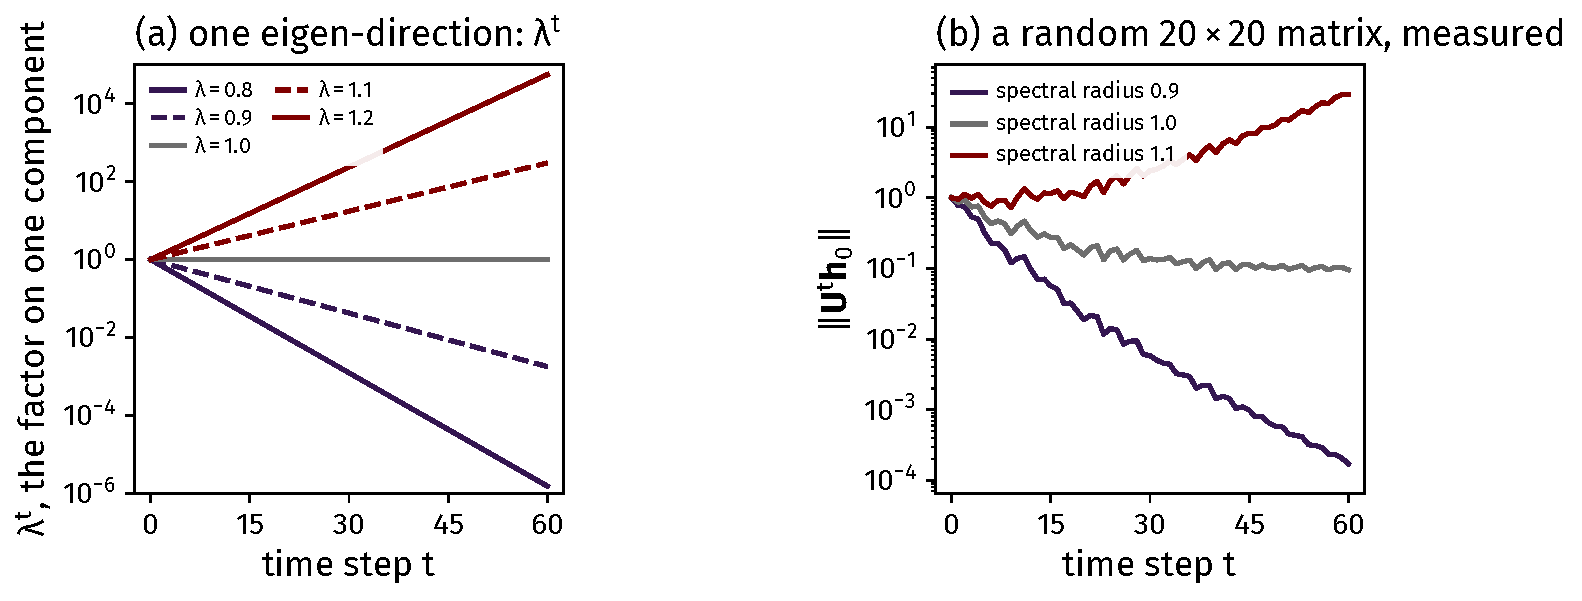
\includegraphics[width=0.84\linewidth]{power_iteration}
  \end{center}
  \vspace{-0.6em}
  {\tiny\color{mcMuted}
  (a) The theorem, one eigen-direction at a time: $\lambda^t$ on a log
  scale is a straight line, down for $|\lambda| < 1$ and up for
  $|\lambda| > 1$; at $60$ steps the two sides differ by ten orders of
  magnitude. (b) The random matrix, measured: at spectral radius $0.9$
  the norm is $1.7 \times 10^{-4}$ after $60$ steps, at $1.1$ it is $29$,
  at $1.0$ it settles near $0.1$ --- the largest component survives
  while the others decay. The wobble early on is the components that
  have not died yet; the slope afterwards is the largest eigenvalue's.
  \hfill Goodfellow et al.\ (2016), Eqs.~10.36--10.39.\par}
\end{frame}

\begin{frame}{The composition, drawn}
  \begin{center}
    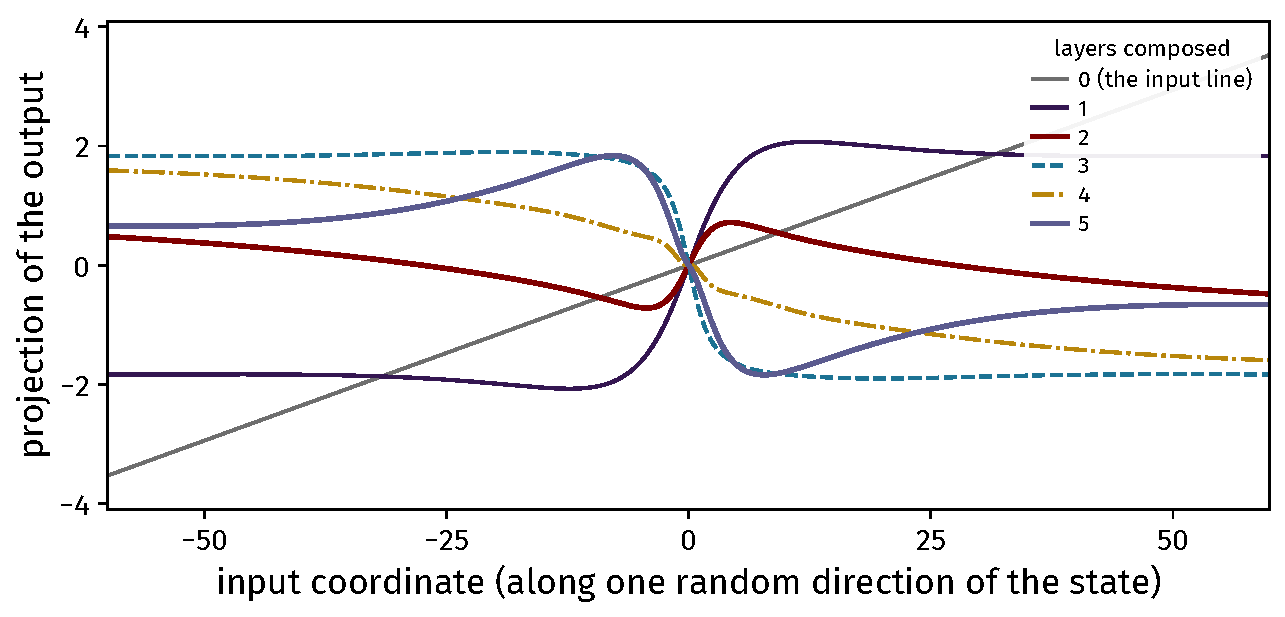
\includegraphics[width=0.72\linewidth]{composition}
  \end{center}
  \vspace{-0.5em}
  {\tiny\color{mcMuted}
  Now with the $\tanh$, recomputed in the layout of Goodfellow's
  Fig.~10.15: a random linear--$\tanh$ layer applied $1$ to $5$ times to a
  $100$-dimensional state, seen along one random line through the state
  (the input coordinate) and projected to one number. The line itself is
  the grey ramp; after one layer it is already an S; after five it is
  flat almost everywhere --- a tiny derivative --- and steep in a few
  places, with more alternations each time. This is the surface the
  gradient must cross, once per step, backwards.
  \hfill Layout of Goodfellow et al.\ (2016), Fig.~10.15, \S10.7.\par}
\end{frame}
\begin{frame}{With the nonlinearity: a bound on the gradient}
  \vspace{-0.45em}
  \begin{propx}[Sufficient condition for vanishing]\label{th:bound}
    \small
    For $\mathbf{h}_t = g(\mathbf{U}\mathbf{h}_{t-1} + \mathbf{W}\mathbf{x}_t)$ with
    $|g'| \leq \gamma$ everywhere ($\gamma = 1$ for $\tanh$, $\tfrac14$ for
    the sigmoid),
    \[
      \Big\| \frac{\partial\mathbf{h}_t}{\partial\mathbf{h}_k} \Big\|
      = \Big\| \prod_{s=k+1}^{t} \mathbf{J}_s \Big\|
      \leq \big( \gamma\,\|\mathbf{U}\| \big)^{t-k},
    \]
    so if $\|\mathbf{U}\| < 1/\gamma$ the gradient from $t$ back to $k$
    vanishes geometrically in the lag.
  \end{propx}
  \vspace{-0.15em}
  {\footnotesize
  \begin{itemize}\itemsep0.12em
    \item \focus{1}{Proof. $\mathbf{J}_s = \mathrm{diag}(g')\,\mathbf{U}$ by the
          chain rule of Class 26, so $\|\mathbf{J}_s\| \leq \gamma\|\mathbf{U}\|$;
          the norm of a product is at most the product of the norms.
          \hfill $\square$}
    \item \focus{2}{Sufficient, not necessary: it says when the gradient
          \emph{must} vanish. Either way a distant cause gets an
          exponentially smaller gradient than a recent one.}
  \end{itemize}}
  \vspace{-0.3em}
  \srcline{Pascanu, Mikolov \& Bengio (2013); Goodfellow et al.\ (2016), \S10.7; Bengio et al.\ (1994).}
\end{frame}

\begin{frame}{The gradient by lag, measured}
  \begin{center}
    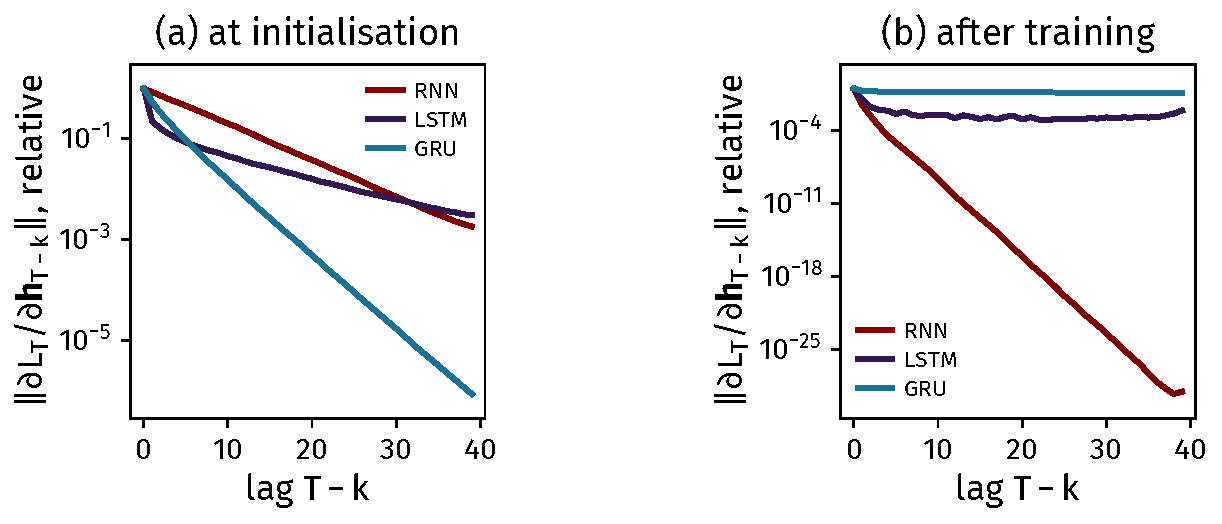
\includegraphics[width=0.80\linewidth]{gradient_lag}
  \end{center}
  \vspace{-0.7em}
  {\tiny\color{mcMuted}
  The corollary of Class 26, measured on three cells --- the two gated
  ones are the next sections' --- of width $32$, trained here to recall
  the first symbol of a sequence at its last step: the running
  sentence's shape, \emph{flights} to \emph{were}, at lag $40$.
  $\|\partial L_T/\partial\mathbf{h}_{T-k}\|$ against the lag $k$, read off
  the tape. (a) At initialisation all three fall with the lag. (b) After
  training the simple RNN's gradient at the first step is $10^{-30}$ of
  its value at the last --- nothing from \emph{were} reaches
  \emph{flights} --- while the LSTM's is $10^{-2}$ and the GRU's $0.4$:
  the gated cells have learned a path along which it survives.
  \hfill Goodfellow et al.\ (2016), \S10.7; Jurafsky \& Martin (2026), \S14.5.\par}
\end{frame}

% =====================================================================
\section{Paths Through Time}
% =====================================================================

\begin{frame}{Three ways to a path the gradient survives}
  \vspace{0.05em}
  {\footnotesize
  \begin{itemize}\itemsep0.25em
    \item The two sections so far say: the only path from \emph{flights}
          to \emph{were} runs through $\mathbf{U}$ and a $\tanh$ at every
          step, and along it the gradient's factors multiply to nothing.
          Every fix is the same fix: build a \alert{second path} whose
          factors stay near one
    \item Three ways to build it, from the books, in order of
          how much they leave to the network:
          \alert{skip connections} shorten the path (fewer factors);
          a \alert{leaky unit} adds a wire with a fixed factor near one;
          a \alert{gate} adds the same wire and lets the network set the
          factor at every step
    \item There is also a way to give up: \alert{echo state networks}
          fix $\mathbf{U}$ at a chosen spectral radius, never train it, and
          learn only the read-out --- a convex problem, and no gradient
          through time at all
  \end{itemize}}
  \srcline{Goodfellow et al.\ (2016), \S10.8--10.10; Lin et al.\ (1996); Mozer (1992); Jaeger \& Haas (2004).}
\end{frame}

\begin{frame}{The three paths, drawn}
  \vspace{-0.3em}
  \begin{center}
    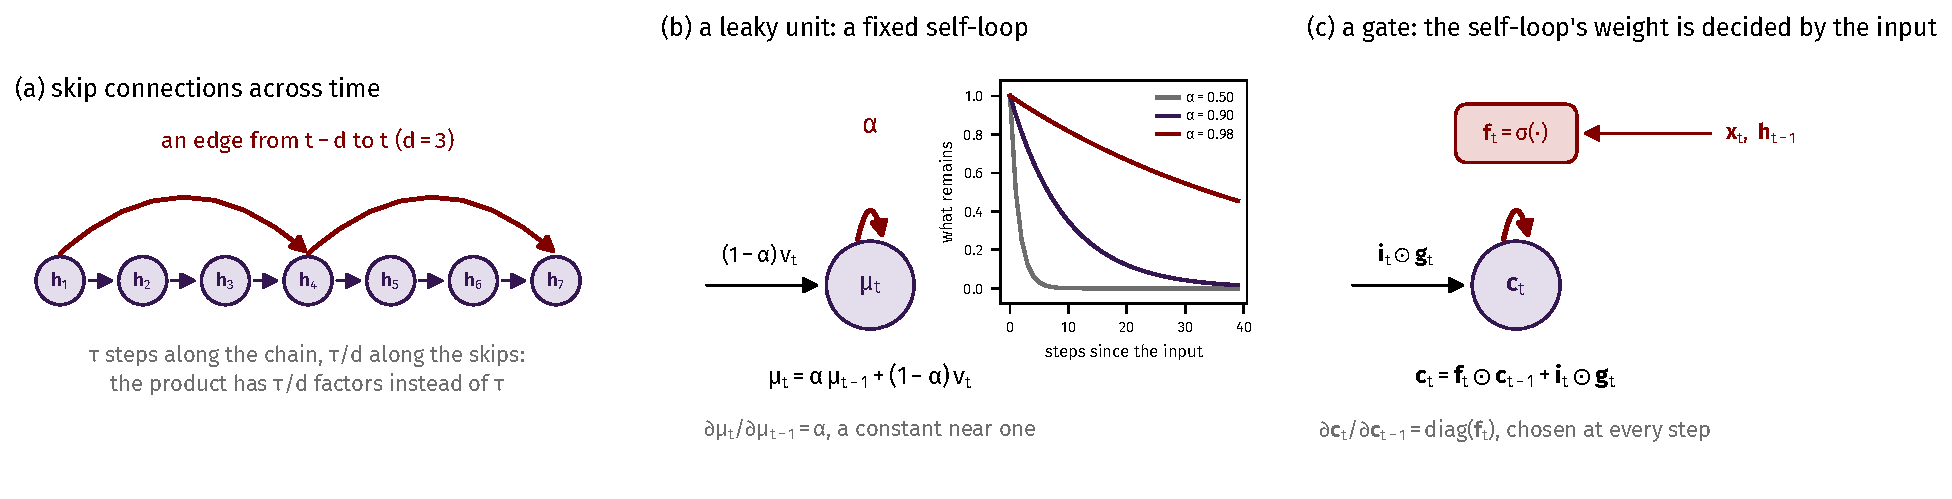
\includegraphics[width=0.98\linewidth]{gradient_paths}
  \end{center}
  \vspace{-0.5em}
  {\tiny\color{mcMuted}
  (a) Skip connections across time: an extra edge from $\mathbf{h}_{t-d}$
  to $\mathbf{h}_t$, so a fact and its gradient cross $\tau$ steps in
  $\tau/d$ hops --- fewer factors in the product, but $d$ is fixed by hand.
  (b) A leaky unit: a linear self-loop of weight $\alpha$, so
  $\partial\mu_t/\partial\mu_{t-1} = \alpha$ exactly, a constant near one;
  the inset shows how much of an input remains after $t$ steps for three
  $\alpha$ --- one fixed time scale per unit. (c) A gate: the same
  self-loop, but its weight $\mathbf{f}_t$ is a sigmoid the network computes
  from $\mathbf{x}_t$ and $\mathbf{h}_{t-1}$ at every step: keep this fact now,
  drop it later. The LSTM's cell line is exactly (c).
  \hfill Goodfellow et al.\ (2016), \S10.8, \S10.9.2, \S10.10; Lin et al.\ (1996); Mozer (1992).\par}
\end{frame}
\begin{frame}{The leaky unit is a running average}
  \vspace{-0.45em}
  \begin{propx}[Time constant of a leaky unit]\label{th:leaky}
    \small
    The unit $\mu_t = \alpha\mu_{t-1} + (1-\alpha)v_t$ unrolls to
    $\mu_t = (1-\alpha)\sum_{s \leq t} \alpha^{\,t-s}\, v_s$:
    geometric weights with time constant $1/(1-\alpha)$ steps.
  \end{propx}
  \vspace{-0.3em}
  \begin{columns}[T, onlytextwidth]
    \begin{column}{0.50\textwidth}
      \vspace{0.1em}
      {\footnotesize
      \begin{itemize}\itemsep0.12em
        \item \focus{1}{Proof. Substitute the recurrence into itself;
              the weights sum to one. \hfill $\square$}
        \item \focus{2}{Along the self-connection
              $\partial\mu_t/\partial\mu_{t-1} = \alpha$, a constant
              near one: the path the gradient survives.}
        \item \focus{3}{A gate replaces the constant $\alpha$ by a
              number in $(0, 1)$ computed at each step.}
      \end{itemize}}
    \end{column}
    \begin{column}{0.48\textwidth}
      \vspace{-0.2em}
      \begin{center}
        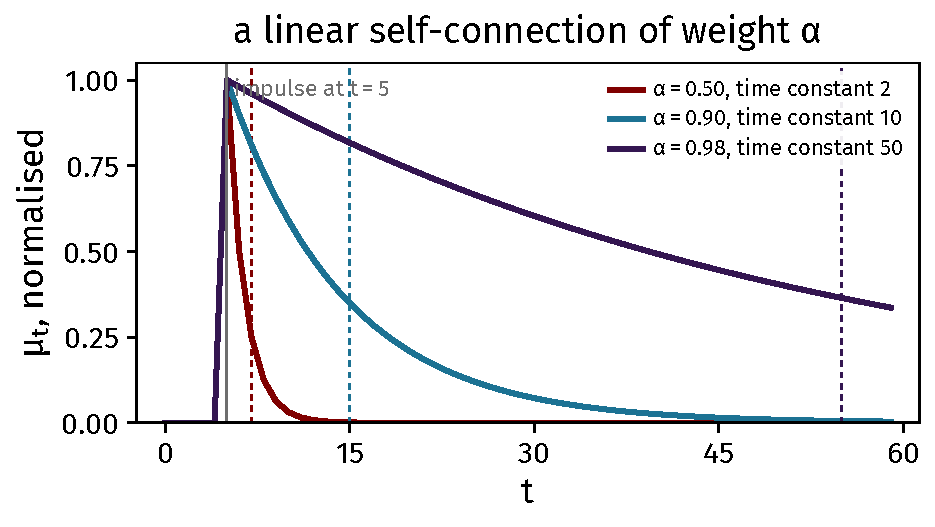
\includegraphics[width=0.74\linewidth]{leaky_unit}
      \end{center}
    \end{column}
  \end{columns}
  \vspace{-0.5em}
  \srcline{Goodfellow et al.\ (2016), \S10.9.2; Mozer (1992).}
\end{frame}

% =====================================================================
\section{The LSTM}
% =====================================================================

\begin{frame}{What the LSTM has to do}
  \vspace{0.05em}
  {\footnotesize
  \begin{itemize}\itemsep0.30em
    \item Take the notebook idea and make it a cell. Two vectors: the
          \alert{cell} $\mathbf{c}_t$, which carries context along a copied
          line, and the \alert{hidden state} $\mathbf{h}_t$, which serves the
          current output as before. Two jobs, two vectors
    \item Manage the cell explicitly with three gates, each the same
          design: a feedforward layer of $\mathbf{x}_t$ and $\mathbf{h}_{t-1}$, a
          sigmoid, and a pointwise product with the thing gated. The
          \alert{forget gate} is the eraser, the \alert{add gate} the pen,
          the \alert{output gate} the lens
    \item The cell's own update is additive,
          $\mathbf{c}_t = \mathbf{f}_t \odot \mathbf{c}_{t-1} + (\text{what is written})$:
          the leaky unit of the last section with $\alpha$ replaced by a
          gate the network sets
    \item First the picture, then the equations, then why it works
  \end{itemize}}
  \srcline{Jurafsky \& Martin (2026), \S14.5; Hochreiter \& Schmidhuber (1997); Gers et al.\ (2000).}
\end{frame}

\begin{frame}{The LSTM cell, drawn}
  \vspace{-0.4em}
  \begin{center}
    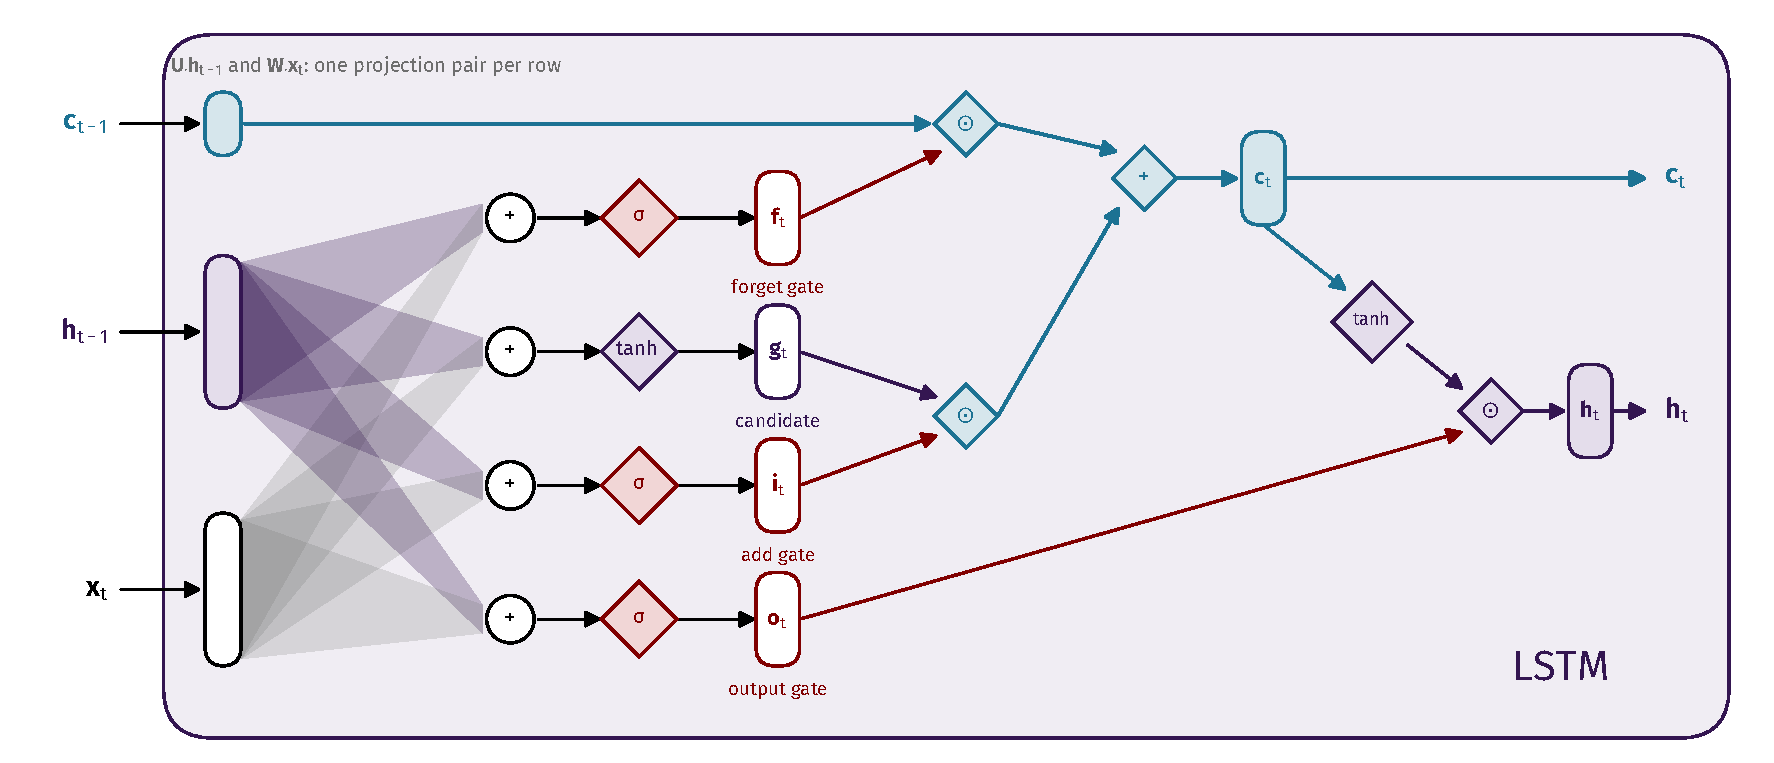
\includegraphics[width=0.86\linewidth]{lstm_cell}
  \end{center}
  \vspace{-0.6em}
  {\tiny\color{mcMuted}
  One LSTM unit as a computation graph. In from the left: $\mathbf{c}_{t-1}$,
  $\mathbf{h}_{t-1}$, $\mathbf{x}_t$. The shaded fans are the projections
  $\mathbf{U}_{\bullet}\mathbf{h}_{t-1}$ and $\mathbf{W}_{\bullet}\mathbf{x}_t$, one pair
  per row, summed and squashed into the forget gate $\mathbf{f}_t$, the
  candidate $\mathbf{g}_t$, the add gate $\mathbf{i}_t$ and the output gate
  $\mathbf{o}_t$. Along the top, the cell line (teal): $\mathbf{c}_{t-1}$ times
  $\mathbf{f}_t$, plus $\mathbf{i}_t \odot \mathbf{g}_t$, is $\mathbf{c}_t$ --- no weight
  matrix on that path. $\mathbf{h}_t$ is $\tanh(\mathbf{c}_t)$ let through by
  $\mathbf{o}_t$. Out on the right: $\mathbf{c}_t$ and $\mathbf{h}_t$.
  \hfill Layout of Jurafsky \& Martin (2026), Fig.~14.13.\par}
\end{frame}
\begin{frame}{The LSTM cell, in equations}
  \vspace{-0.3em}
  \begin{defx}[LSTM]\label{th:lstm}
    \small
    \[
      \begin{aligned}
        \mathbf{f}_t &= \sigma(\mathbf{U}_f\mathbf{h}_{t-1} + \mathbf{W}_f\mathbf{x}_t) &&\text{forget gate} \qquad
        &\mathbf{k}_t &= \mathbf{c}_{t-1} \odot \mathbf{f}_t &&\text{what survives}\\
        \mathbf{g}_t &= \tanh(\mathbf{U}_g\mathbf{h}_{t-1} + \mathbf{W}_g\mathbf{x}_t) &&\text{candidate}
        &\mathbf{i}_t &= \sigma(\mathbf{U}_i\mathbf{h}_{t-1} + \mathbf{W}_i\mathbf{x}_t) &&\text{add gate}\\
        \mathbf{j}_t &= \mathbf{g}_t \odot \mathbf{i}_t &&\text{what is added}
        &\mathbf{c}_t &= \mathbf{j}_t + \mathbf{k}_t &&\text{new cell}\\
        \mathbf{o}_t &= \sigma(\mathbf{U}_o\mathbf{h}_{t-1} + \mathbf{W}_o\mathbf{x}_t) &&\text{output gate}
        &\mathbf{h}_t &= \mathbf{o}_t \odot \tanh(\mathbf{c}_t) &&\text{new hidden}
      \end{aligned}
    \]
  \end{defx}
  \vspace{-0.15em}
  {\footnotesize
  \begin{itemize}\itemsep0.12em
    \item The picture, line by line: the eraser $\mathbf{f}_t$ decides what
          of $\mathbf{c}_{t-1}$ survives; the pen writes $\mathbf{g}_t$, as much as
          $\mathbf{i}_t$ allows; the lens $\mathbf{o}_t$ decides what is read into
          $\mathbf{h}_t$. Four weight pairs instead of one; a forget bias of
          $1$ makes the cell start by remembering
  \end{itemize}}
  \vspace{-0.3em}
  \srcline{Jurafsky \& Martin (2026), Eqs.~14.20--14.27; Goodfellow et al.\ (2016), Eqs.~10.40--10.44.}
\end{frame}

\begin{frame}{The LSTM cell, as a block diagram}
  \vspace{-0.4em}
  \begin{center}
    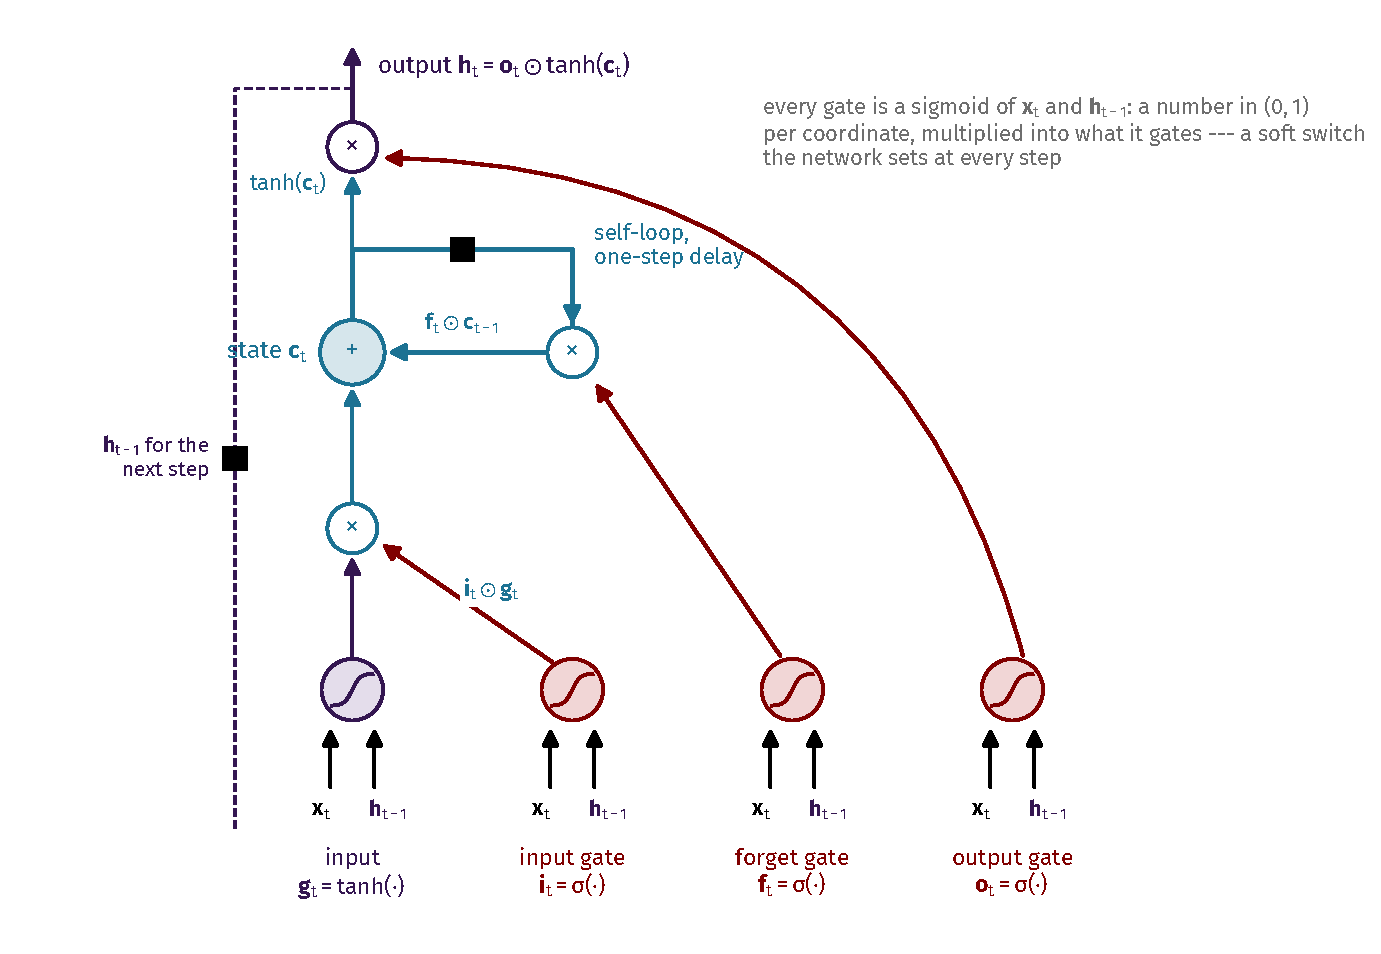
\includegraphics[height=0.58\textheight]{lstm_block}
  \end{center}
  \vspace{-0.6em}
  {\tiny\color{mcMuted}
  Goodfellow's view of the same cell, in the layout of his Fig.~10.16.
  Along the bottom, four units, each fed by $\mathbf{x}_t$ and $\mathbf{h}_{t-1}$:
  the input unit (a $\tanh$, the candidate) and three sigmoid gates. The
  input is multiplied by the input gate and added into the state; the
  state has a linear self-loop through a one-step delay (black square)
  whose weight is the forget gate; the state, through a $\tanh$, is
  multiplied by the output gate to give the output, which is next step's
  $\mathbf{h}_{t-1}$ (dashed). A gate is a number in $(0, 1)$ per
  coordinate, multiplied into what it gates: a soft switch the network
  sets at every step.
  \hfill Layout of Goodfellow et al.\ (2016), Fig.~10.16, \S10.10.1.\par}
\end{frame}
\begin{frame}{Why the cell remembers}
  \vspace{-0.45em}
  \begin{propx}[The cell's gradient is a product of forget gates]\label{th:carousel}
    \small
    Holding the gates fixed, along the cell's own path
    $\ \partial\mathbf{c}_t/\partial\mathbf{c}_k = \prod_{s=k+1}^{t} \mathrm{diag}(\mathbf{f}_s)$,
    a product of numbers in $(0, 1)$ with \emph{no weight matrix and no
    activation derivative} in it: with $\mathbf{f}_s \approx \mathbf{1}$ the
    gradient passes unattenuated.
  \end{propx}
  \vspace{-0.15em}
  {\footnotesize
  \begin{itemize}\itemsep0.12em
    \item \focus{1}{Proof. $\mathbf{c}_s = \mathbf{f}_s \odot \mathbf{c}_{s-1} + \mathbf{j}_s$
          is linear in $\mathbf{c}_{s-1}$ with coefficient $\mathbf{f}_s$;
          chain the steps. \hfill $\square$}
    \item \focus{2}{Against Proposition~\ref{th:bound}: the simple
          cell's factor $\mathrm{diag}(g')\,\mathbf{U}$ is typically well
          below one; the LSTM's is a gate the network can hold at one
          --- the \alert{constant error carousel}. On the sentence: with
          $\mathbf{f}_s \approx \mathbf{1}$ from \emph{flights} to \emph{were}, the
          loss at \emph{were} reaches the write at \emph{flights} intact.
          The gates depend on $\mathbf{h}_{t-1}$ too, so there are other
          paths; this is the one that survives.}
  \end{itemize}}
  \vspace{-0.3em}
  \srcline{Hochreiter \& Schmidhuber (1997); Gers et al.\ (2000); Goodfellow et al.\ (2016), \S10.10.1.}
\end{frame}


\begin{frame}{Gated units are drop-in modules}
  \vspace{-0.3em}
  \begin{center}
    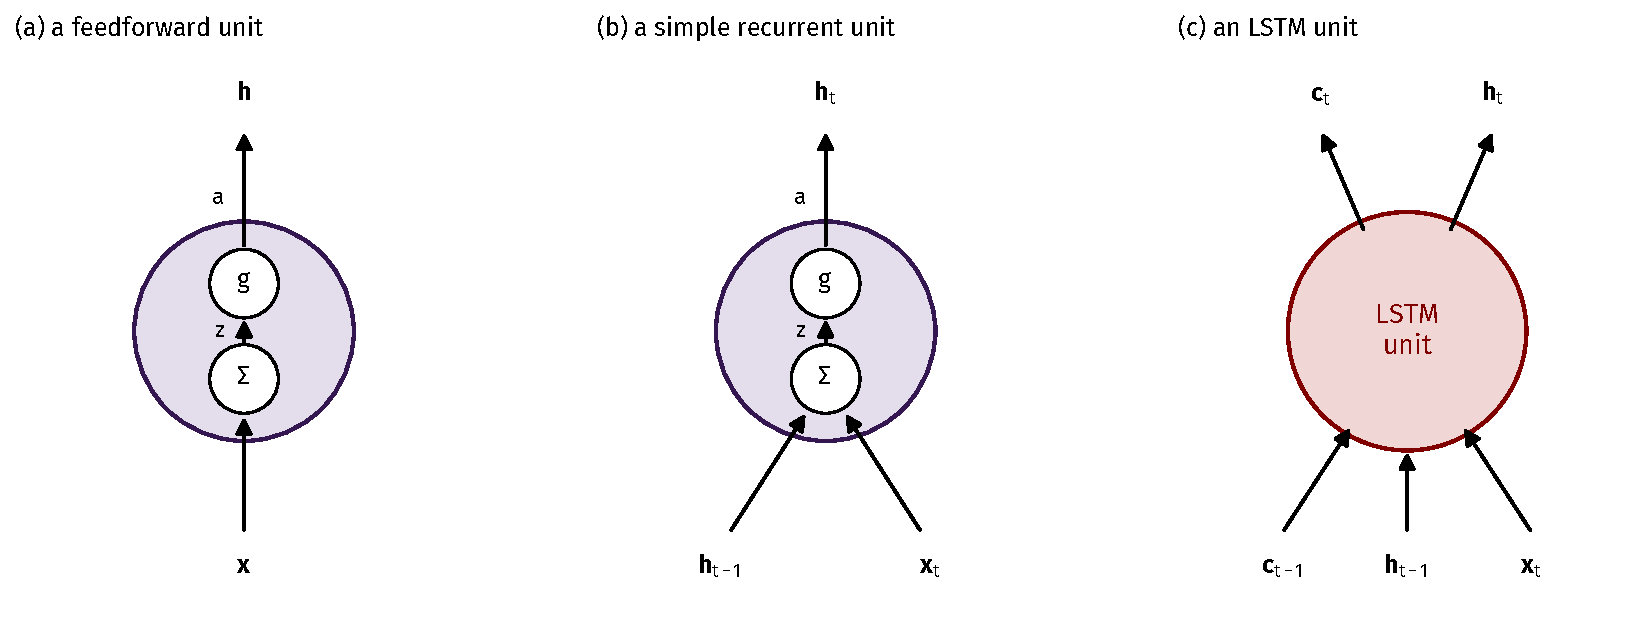
\includegraphics[width=0.74\linewidth]{dropin_modules}
  \end{center}
  \vspace{-0.5em}
  {\tiny\color{mcMuted}
  The three units side by side, in the layout of Jurafsky's Fig.~14.14.
  (a) A feedforward unit: a weighted sum $z$, an activation $g$, an output.
  (b) A simple recurrent unit: the same with two inputs, $\mathbf{h}_{t-1}$
  and $\mathbf{x}_t$. (c) An LSTM unit: everything of the last two slides is
  inside the circle; from outside, the only change is a second vector in,
  $\mathbf{c}_{t-1}$, and a second vector out, $\mathbf{c}_t$. So an LSTM drops
  into every architecture of Classes 27 and 29 --- encoder, decoder,
  stacked, bidirectional --- and is unrolled and trained exactly as in
  Class 26.
  \hfill Layout of Jurafsky \& Martin (2026), Fig.~14.14, \S14.5.1.\par}
\end{frame}

% =====================================================================
\section{Other Gated Cells}
% =====================================================================

\begin{frame}{The gated recurrent unit}
  \vspace{-0.45em}
  \begin{defx}[GRU]\label{th:gru}
    \small
    One gate decides both what to forget and what to write:
    \[
      \begin{aligned}
        \mathbf{u}_t &= \sigma(\mathbf{U}_u\mathbf{h}_{t-1} + \mathbf{W}_u\mathbf{x}_t) &&\text{update gate}\\
        \mathbf{r}_t &= \sigma(\mathbf{U}_r\mathbf{h}_{t-1} + \mathbf{W}_r\mathbf{x}_t) &&\text{reset gate}\\
        \tilde{\mathbf{h}}_t &= \tanh\big(\mathbf{U}_h(\mathbf{r}_t \odot \mathbf{h}_{t-1}) + \mathbf{W}_h\mathbf{x}_t\big) &&\text{candidate}\\
        \mathbf{h}_t &= \mathbf{u}_t \odot \mathbf{h}_{t-1} + (\mathbf{1} - \mathbf{u}_t) \odot \tilde{\mathbf{h}}_t &&\text{new state}
      \end{aligned}
    \]
  \end{defx}
  \vspace{-0.15em}
  {\footnotesize
  \begin{itemize}\itemsep0.12em
    \item The same idea with less equipment: no separate notebook,
          three weight pairs against four. The update gate $\mathbf{u}_t$
          is eraser and pen in one --- what is kept of the old state is
          exactly what is not overwritten by the new; the reset gate
          chooses what of the past the candidate may see
  \end{itemize}}
  \vspace{-0.3em}
  \srcline{Goodfellow et al.\ (2016), Eqs.~10.45--10.47; Cho et al.\ (2014); Chung et al.\ (2014).}
\end{frame}

\begin{frame}{The GRU's state stays between old and new}
  \vspace{-0.3em}
  \begin{propx}[Convex update]\label{th:convex}
    \small
    Since every entry of $\mathbf{u}_t$ lies in $(0, 1)$, each coordinate of
    $\mathbf{h}_t = \mathbf{u}_t \odot \mathbf{h}_{t-1} + (\mathbf{1} - \mathbf{u}_t) \odot \tilde{\mathbf{h}}_t$
    lies between the old state and the candidate. Along the old state the
    derivative is $\mathrm{diag}(\mathbf{u}_t)$, so a coordinate with
    $u \approx 1$ is copied unchanged and its gradient passes unchanged,
    exactly as on the LSTM's cell line.
  \end{propx}
  \vspace{0.1em}
  {\footnotesize
  \begin{itemize}\itemsep0.24em
    \item \focus{1}{Proof. $u\,a + (1-u)\,b$ with $u \in (0, 1)$ is a
          convex combination of $a$ and $b$; differentiate in $a$.
          \hfill $\square$}
    \item \focus{2}{Which pieces of the LSTM are needed? Ablations
          find no variant that beats both LSTM and GRU across tasks;
          the forget gate is the crucial ingredient, and a forget bias of
          $1$ makes the LSTM as strong as the best variant.}
  \end{itemize}}
  \srcline{Goodfellow et al.\ (2016), \S10.10.2; Greff et al.\ (2017); Jozefowicz et al.\ (2015).}
\end{frame}

\begin{frame}{Three cells on one task}
  \begin{center}
    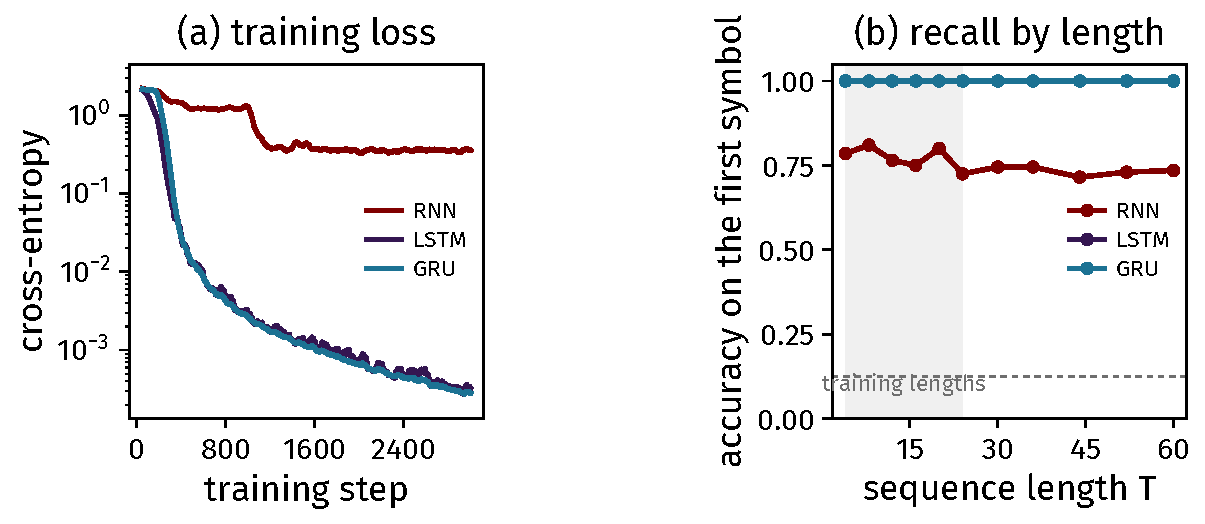
\includegraphics[width=0.86\linewidth]{long_dependency}
  \end{center}
  \vspace{-0.7em}
  {\tiny\color{mcMuted}
  The recall task --- the sentence's shape, a fact at the first step
  needed at the last --- on an RNN, an LSTM and a GRU of width $32$,
  trained the same way for $3{,}000$ steps on lengths $4$--$24$. (a)
  Training loss: the gated cells reach zero, the simple cell does not.
  (b) Accuracy by sequence length, tested to $60$: the gated cells are
  perfect at every length, including far beyond what they trained on;
  the simple RNN never passes $81\%$, even at length $8$. Chance is $1/8$.
  \hfill Jurafsky \& Martin (2026), \S14.5; Goodfellow et al.\ (2016), \S10.10.\par}
\end{frame}

% =====================================================================
\section{Optimising Through Time}
% =====================================================================

\begin{frame}{Clipping the gradient}
  \vspace{-0.45em}
  \begin{propx}[Norm clipping keeps the direction]\label{th:clip}
    \small
    Replace the gradient $\mathbf{g}$ by
    \[
      \mathbf{g} \leftarrow \frac{\mathbf{g}\,v}{\|\mathbf{g}\|} \quad \text{if } \|\mathbf{g}\| > v .
    \]
    The step is still along $\mathbf{g}$, a descent direction, and its
    length is at most $\eta v$ whatever the gradient's size.
  \end{propx}
  \vspace{0.05em}
  {\footnotesize
  \begin{itemize}\itemsep0.2em
    \item \focus{1}{Proof. A positive scaling changes length only, and
          $\|\eta\mathbf{g}v/\|\mathbf{g}\|\| = \eta v$. \hfill $\square$}
    \item \focus{2}{Why: the loss over many steps has \alert{cliffs},
          flat regions separated by walls exponentially steep in the
          number of steps, since $\mathbf{U}$ multiplies itself once per
          step; one step at a cliff can undo all the descent so far.
          Clipping addresses explosion only.}
  \end{itemize}}
  \vspace{-0.3em}
  \srcline{Goodfellow et al.\ (2016), \S10.11.1, Eqs.~10.48--10.49; Pascanu et al.\ (2013); Mikolov (2012).}
\end{frame}

\begin{frame}{Clipping at a cliff, drawn}
  \vspace{-0.3em}
  \begin{center}
    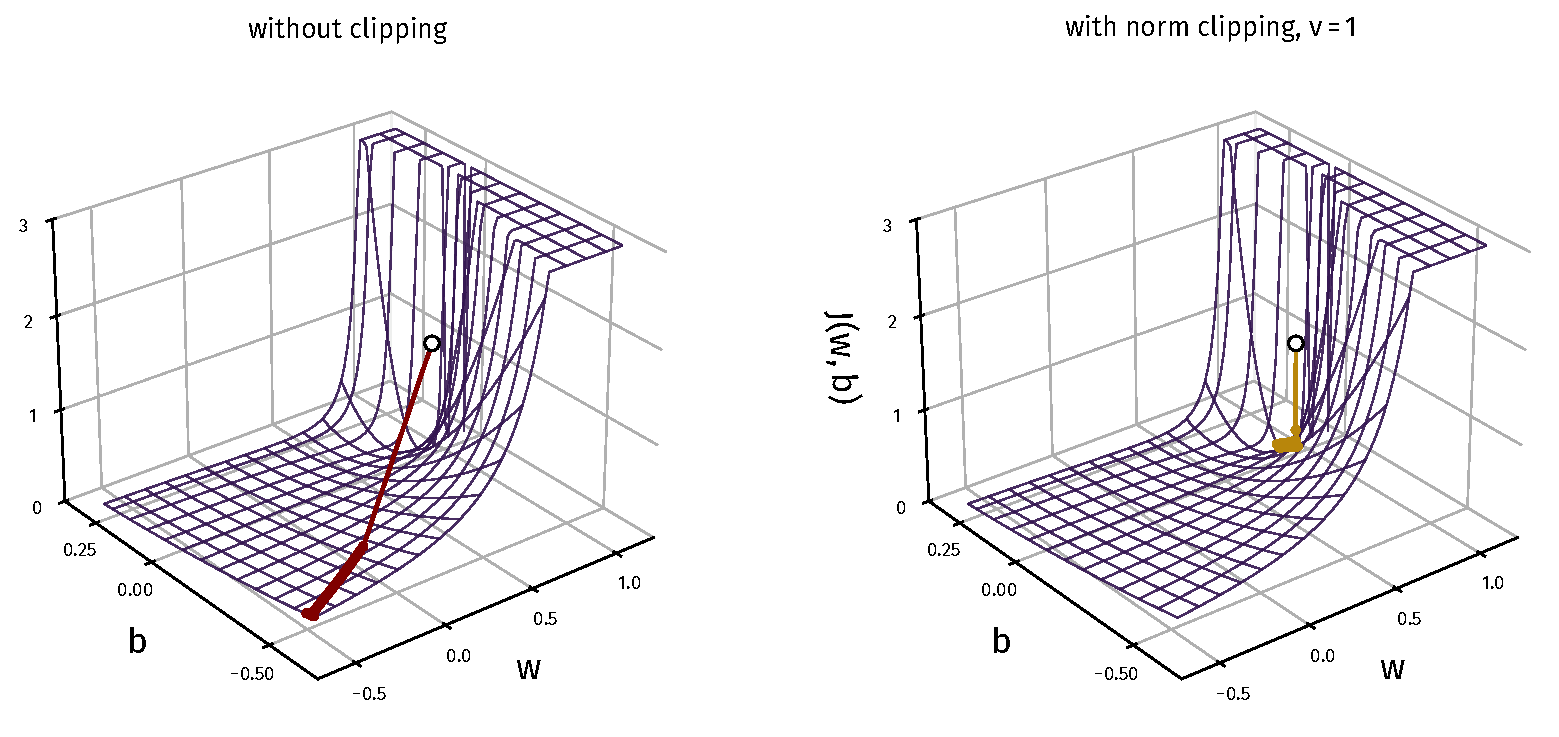
\includegraphics[width=0.74\linewidth]{clipping}
  \end{center}
  \vspace{-0.6em}
  {\tiny\color{mcMuted}
  The loss surface $J(w, b)$ of a recurrent net with two parameters,
  $h_t = w\,h_{t-1} + b$ for $50$ steps and a squared error at the end,
  computed here and drawn in the layout of Goodfellow's Fig.~10.17: flat
  almost everywhere and exponentially steep at $w \approx 1$, because
  $w$ multiplies itself once per step. Gradient descent from the same
  start on the lip of the cliff, with the same step size: without
  clipping (left) the first step at the cliff throws the parameters out
  of the frame, to a loss of $0.36$; with the norm clipped at $v = 1$
  (right) the steps are bounded and settle in the ravine at $0.005$.
  \hfill Layout of Goodfellow et al.\ (2016), Fig.~10.17, after Pascanu et al.\ (2013).\par}
\end{frame}
\begin{frame}{Encouraging the gradient to flow}
  \vspace{0.05em}
  {\footnotesize
  \begin{itemize}\itemsep0.30em
    \item Clipping handles explosion; vanishing needs a path whose
          product of derivatives is near one --- the gates --- or a
          \alert{regulariser} that asks for it
    \item Pascanu et al.\ penalise, at every step, how much the
          back-propagated gradient shrinks in crossing that step:
          \[
            \Omega = \sum_t \left(
              \frac{\big\| (\nabla_{\mathbf{h}_t}L)^{\mathsf T}\,\partial\mathbf{h}_t/\partial\mathbf{h}_{t-1} \big\|}
                   {\|\nabla_{\mathbf{h}_t}L\|} - 1 \right)^2 ,
          \]
          treating $\nabla_{\mathbf{h}_t}L$ as a constant for the purpose
          of the regulariser
    \item With clipping alongside it, this lengthens the dependencies a
          simple RNN can learn; with abundant data it is not as
          effective as an LSTM, which is why the gate won
  \end{itemize}}
  \srcline{Goodfellow et al.\ (2016), \S10.11.2, Eqs.~10.50--10.52; Pascanu et al.\ (2013).}
\end{frame}

\begin{frame}{Where the gate leads: explicit memory, drawn}
  \vspace{-0.3em}
  \begin{center}
    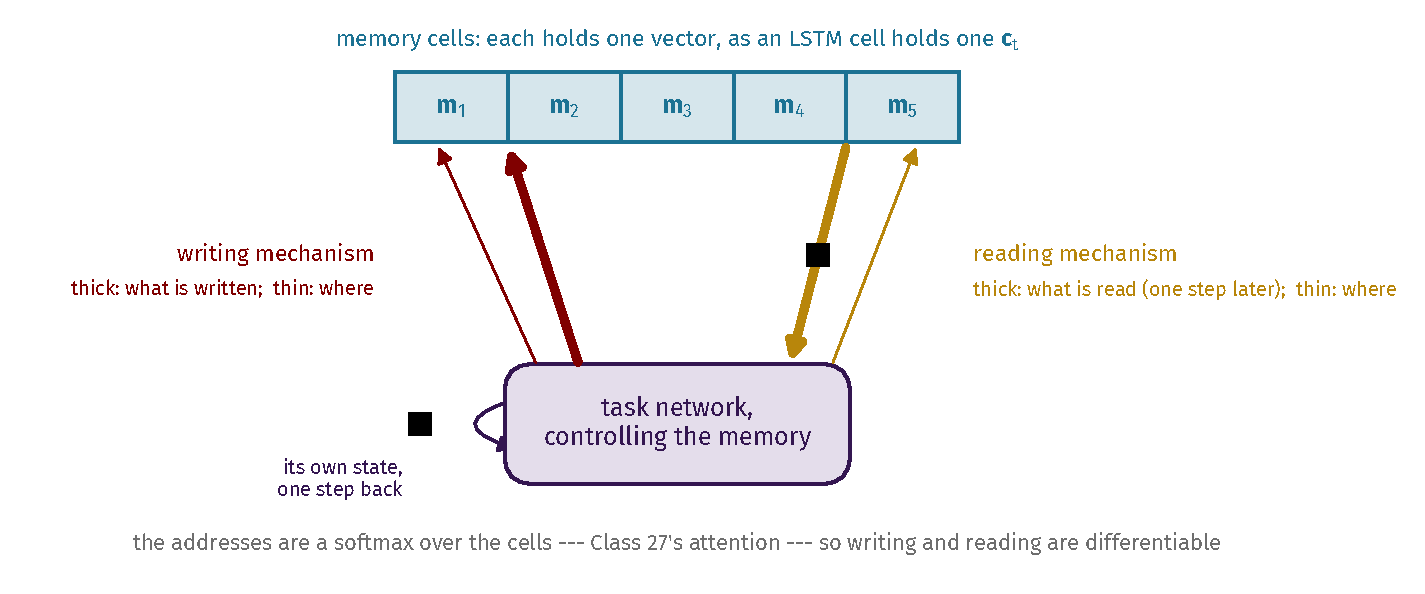
\includegraphics[width=0.84\linewidth]{explicit_memory}
  \end{center}
  \vspace{-0.5em}
  {\tiny\color{mcMuted}
  A network with an explicit memory, in the layout of Goodfellow's
  Fig.~10.18: a row of memory cells, each holding one vector; a task
  network with its own recurrence (the black square is a one-step delay)
  that controls a writing mechanism and a reading mechanism. Thick arrows
  carry the content written and read; thin arrows carry the addresses
  the task network chooses.
  \hfill Layout of Goodfellow et al.\ (2016), Fig.~10.18.\par}
\end{frame}

\begin{frame}{Where the gate leads: explicit memory, explained}
  \vspace{-0.1em}
  {\footnotesize
  \begin{itemize}\itemsep0.28em
    \item An LSTM cell is a memory of \alert{one} vector with a learned
          pen, eraser and lens. Build the memory as a \alert{set} of such
          cells: Weston et al.'s memory networks, Graves et al.'s neural
          Turing machine
    \item \alert{Writing.} The task network produces a vector to store
          and a soft address: a softmax over the cells, so the write lands
          mostly in one cell and a little in the others. The pen of the
          LSTM, with a choice of page
    \item \alert{Reading.} The same: a softmax over the cells, and the
          content read is the weighted average of what they hold ---
          Class 27's attention, over memory instead of over encoder
          states. Because the address is a softmax and not an index, the
          whole thing is differentiable and trains end to end
    \item \alert{Why it helps.} A fact is stored in one write and kept
          until overwritten; on the sentence, \emph{flights, plural} goes
          into a cell at word two and is read back at word seven, whatever
          happened in between
  \end{itemize}}
  \srcline{Goodfellow et al.\ (2016), \S10.12; Weston et al.\ (2014); Graves et al.\ (2014); Class 27.}
\end{frame}

% =====================================================================
\section{Putting It Together}
% =====================================================================

\begin{frame}{The cell, opened}
  \vspace{0.2em}
  {\scriptsize
  \renewcommand{\arraystretch}{1.36}
  \begin{tabular}{@{}l@{\hspace{1.0em}}l@{\hspace{1.0em}}l@{\hspace{1.0em}}l@{}}
    & \textbf{state} & \textbf{path across time} & \textbf{derivative along it}\\
    simple RNN & $\mathbf{h}_t$ & through $\mathbf{U}$ and $g$ every step & $\mathrm{diag}(g')\,\mathbf{U}$, shrinks or explodes\\
    leaky unit & $\mu_t$ & a linear self-connection & the constant $\alpha$\\
    LSTM & $\mathbf{h}_t$ and $\mathbf{c}_t$ & the cell line & $\mathrm{diag}(\mathbf{f}_t)$, chosen by the network\\
    GRU & $\mathbf{h}_t$ & the update gate's copy & $\mathrm{diag}(\mathbf{u}_t)$, chosen by the network\\
  \end{tabular}}
  \vspace{0.6em}

  \begin{redhighlight}
    Every fix is the same fix: give the gradient a path whose factors
    stay near one. The gate is the version where the network decides,
    at every step, which facts get that path.
  \end{redhighlight}
\end{frame}

\begin{frame}{Takeaways}
  \vspace{-0.1em}
  {\scriptsize
  \begin{enumerate}\itemsep0.24em
    \item A fact that must survive a long wait, and the gradient that
          would teach it, both cross the same wire once per step; the
          simple cell has one vector, rewritten every step, for keeping
          and for everything else
    \item A repeated linear map raises its eigenvalues to the power of
          the time: components decay or explode geometrically
          (Theorem~\ref{th:power}), and the same product bounds the
          gradient of the nonlinear cell (Proposition~\ref{th:bound})
    \item A linear self-connection of weight near one is a running
          average with a long time constant, and a path the gradient
          survives (Proposition~\ref{th:leaky})
    \item The LSTM adds a copied cell and three gates --- eraser, pen,
          lens (Definition~\ref{th:lstm});
          along the cell line the gradient is a product of forget gates,
          with no weight matrix in it (Proposition~\ref{th:carousel})
    \item The GRU does the same with two gates and no separate cell;
          its update is a convex combination (Definition~\ref{th:gru},
          Proposition~\ref{th:convex})
    \item Norm clipping bounds the step without changing its direction
          (Proposition~\ref{th:clip}); an LSTM is a better answer to
          vanishing than any regulariser
  \end{enumerate}}
  \vspace{-0.2em}
  \bridge{Class 29 puts the cell to work: language models, taggers,
  classifiers, and what stacking and bidirectionality buy.}
\end{frame}

\begin{frame}[allowframebreaks]{References}
  \vspace{0.3em}
  {\scriptsize
  \begin{enumerate}\itemsep0.30em
    \item D.\ Jurafsky \& J.\ H.\ Martin, \emph{Speech and Language
          Processing}, 3rd ed.\ draft, August 2026. Ch.~14 \S14.5
          (Eqs.~14.20--14.27, Figs.~14.13--14.14), \S14.5.1.
    \item I.\ Goodfellow, Y.\ Bengio \& A.\ Courville, \emph{Deep
          Learning}, MIT Press, 2016. \S10.7 (Eqs.~10.36--10.39,
          Fig.~10.15), \S10.8, \S10.9, \S10.10 (Eqs.~10.40--10.47,
          Fig.~10.16), \S10.11 (Eqs.~10.48--10.52, Fig.~10.17),
          \S10.12 (Fig.~10.18).
    \item S.\ Hochreiter \& J.\ Schmidhuber, ``Long short-term memory'',
          \emph{Neural Computation} 9(8), 1997.
    \item F.\ A.\ Gers, J.\ Schmidhuber \& F.\ Cummins, ``Learning to
          forget: continual prediction with LSTM'', \emph{Neural
          Computation} 12(10), 2000.
    \item Y.\ Bengio, P.\ Simard \& P.\ Frasconi, ``Learning long-term
          dependencies with gradient descent is difficult'', \emph{IEEE
          Trans.\ Neural Networks} 5(2), 1994.
    \item R.\ Pascanu, T.\ Mikolov \& Y.\ Bengio, ``On the difficulty of
          training recurrent neural networks'', ICML 2013.
    \item K.\ Cho et al., ``Learning phrase representations using RNN
          encoder--decoder for statistical machine translation'',
          EMNLP 2014; J.\ Chung et al., ``Empirical evaluation of gated
          recurrent neural networks on sequence modeling'', 2014.
    \item K.\ Greff et al., ``LSTM: a search space odyssey'', \emph{IEEE
          TNNLS} 28(10), 2017; R.\ Jozefowicz, W.\ Zaremba \&
          I.\ Sutskever, ``An empirical exploration of recurrent network
          architectures'', ICML 2015.
    \item M.\ C.\ Mozer, ``Induction of multiscale temporal structure'',
          NeurIPS 1992; T.\ Lin et al., ``Learning long-term dependencies
          in NARX recurrent neural networks'', \emph{IEEE Trans.\ Neural
          Networks} 7(6), 1996.
    \item H.\ Jaeger \& H.\ Haas, ``Harnessing nonlinearity: predicting
          chaotic systems and saving energy in wireless communication'',
          \emph{Science} 304, 2004.
    \item T.\ Mikolov, \emph{Statistical Language Models Based on Neural
          Networks}, PhD thesis, Brno University of Technology, 2012.
    \item J.\ Weston, S.\ Chopra \& A.\ Bordes, ``Memory networks'',
          ICLR 2015 (arXiv 2014); A.\ Graves, G.\ Wayne \& I.\ Danihelka,
          ``Neural Turing machines'', arXiv:1410.5401, 2014.
  \end{enumerate}}
\end{frame}

\begin{frame}[standout]
  Questions?
\end{frame}

\end{document}
